\documentclass{article}
\usepackage{tikz, comment}
\usepackage{pifont}
\usepackage{fontspec}
\usetikzlibrary{arrows, decorations.markings, decorations.pathreplacing}
\begin{comment}
:Title: Not defined yet
:Tags: polar coordinates;moment;pi;;area using polar coordinates, polar integral formula ;polar form of a complex number
:Prob: 0.4417;0.4113;0.3994;0.3926;0.3896
:Slug: No name yet

Description Here.........
\end{comment}
\begin{document}\centering

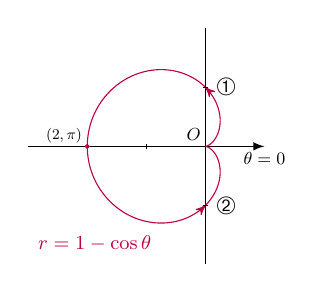
\begin{tikzpicture}[>=latex,xscale=.5*1.5, yscale=.5*1.5][font=\sf\small]

%\draw[xstep=1cm,ystep=1cm,color=gray!80] (0, -1) grid (8, 8);

\draw[->] (-3, 0) -- (1, 0)node[below, scale=0.7] {$\theta=0$};
\draw[] (0, -2) -- (0, 2);

\draw[->, >=stealth', purple, samples=150, smooth, domain=0:pi/2, variable=\t]
plot ({(1-cos(\t r))*cos(\t r)}, {(1-cos(\t r))*sin(\t r)})--({(1-cos(pi/2 r))*cos(pi/2 r)}, {(1-cos(pi/2 r))*sin(pi/2 r)});
\draw[->, >=stealth', purple, samples=150, smooth, domain=pi/2:3*pi/2, variable=\t]
plot ({(1-cos(\t r))*cos(\t r)}, {(1-cos(\t r))*sin(\t r)})--({(1-cos(3*pi/2 r))*cos(3*pi/2 r)}, {(1-cos(3*pi/2 r))*sin(3*pi/2 r)});

\draw[purple, samples=100, smooth, domain=3*pi/2:2*pi, variable=\t]
plot ({(1-cos(\t r))*cos(\t r)}, {(1-cos(\t r))*sin(\t r)});

\draw[purple, fill, xscale=1/1.5, yscale=1/1.5] ({-2*1.5}, {0*1.5}) circle(0.05) node[black, left, xshift=0, yshift=4, scale=0.6] {$(2, \pi)$};

\node[purple, xshift=-40, yshift=-35, scale=0.8] at (0,0) {$r=1-\cos \theta$};

\foreach \x in {-1}
\draw (\x,2pt/1.5) -- (\x,-2pt/1.5)
node[anchor=north] {}%{\tiny$\x$}
;
\foreach \x in {}
\draw (\x,2pt/1.5) -- (\x,-2pt/1.5)
node[anchor=south] {\tiny$\x$}
;
\foreach \y in {-1,1}
\draw (-2pt/1.5,\y) -- (2pt/1.5,\y)
node[anchor=east] {}%{\tiny $\y$}
;

\node at (0.35, 1) {\ding{192}};
\node at (0.35, -1) {\ding{193}};

\node[scale=0.7] at (-0.3/1.5, 0.3/1.5) {$O$};

\end{tikzpicture}
\end{document}